% Options for packages loaded elsewhere
\PassOptionsToPackage{unicode}{hyperref}
\PassOptionsToPackage{hyphens}{url}
\PassOptionsToPackage{dvipsnames,svgnames,x11names}{xcolor}
\documentclass[
  10pt,
  fontset=fandol]{ctexart}
\usepackage{xcolor}
\usepackage[margin=16mm]{geometry}
\usepackage{amsmath,amssymb}
\setcounter{secnumdepth}{-\maxdimen} % remove section numbering
\usepackage{iftex}
\ifPDFTeX
  \usepackage[T1]{fontenc}
  \usepackage[utf8]{inputenc}
  \usepackage{textcomp} % provide euro and other symbols
\else % if luatex or xetex
  \usepackage{unicode-math} % this also loads fontspec
  \defaultfontfeatures{Scale=MatchLowercase}
  \defaultfontfeatures[\rmfamily]{Ligatures=TeX,Scale=1}
\fi
\usepackage{lmodern}
\ifPDFTeX\else
  % xetex/luatex font selection
\fi
% Use upquote if available, for straight quotes in verbatim environments
\IfFileExists{upquote.sty}{\usepackage{upquote}}{}
\IfFileExists{microtype.sty}{% use microtype if available
  \usepackage[]{microtype}
  \UseMicrotypeSet[protrusion]{basicmath} % disable protrusion for tt fonts
}{}
\makeatletter
\@ifundefined{KOMAClassName}{% if non-KOMA class
  \IfFileExists{parskip.sty}{%
    \usepackage{parskip}
  }{% else
    \setlength{\parindent}{0pt}
    \setlength{\parskip}{6pt plus 2pt minus 1pt}}
}{% if KOMA class
  \KOMAoptions{parskip=half}}
\makeatother
\usepackage{longtable,booktabs,array}
\newcounter{none} % for unnumbered tables
\usepackage{calc} % for calculating minipage widths
% Correct order of tables after \paragraph or \subparagraph
\usepackage{etoolbox}
\makeatletter
\patchcmd\longtable{\par}{\if@noskipsec\mbox{}\fi\par}{}{}
\makeatother
% Allow footnotes in longtable head/foot
\IfFileExists{footnotehyper.sty}{\usepackage{footnotehyper}}{\usepackage{footnote}}
\makesavenoteenv{longtable}
\usepackage{graphicx}
\makeatletter
\newsavebox\pandoc@box
\newcommand*\pandocbounded[1]{% scales image to fit in text height/width
  \sbox\pandoc@box{#1}%
  \Gscale@div\@tempa{\textheight}{\dimexpr\ht\pandoc@box+\dp\pandoc@box\relax}%
  \Gscale@div\@tempb{\linewidth}{\wd\pandoc@box}%
  \ifdim\@tempb\p@<\@tempa\p@\let\@tempa\@tempb\fi% select the smaller of both
  \ifdim\@tempa\p@<\p@\scalebox{\@tempa}{\usebox\pandoc@box}%
  \else\usebox{\pandoc@box}%
  \fi%
}
% Set default figure placement to htbp
\def\fps@figure{htbp}
\makeatother
\setlength{\emergencystretch}{3em} % prevent overfull lines
\providecommand{\tightlist}{%
  \setlength{\itemsep}{0pt}\setlength{\parskip}{0pt}}
\usepackage{amsmath,amssymb,mathtools,needspace}
\xeCJKDeclareCharClass{CJK}{"2032,"0400->"04FF,"2160->"216B,"2460->"2473,"25A0,"25C7,"25CB,"25CF}
\IfFontExistsTF{Arial Unicode MS}{\xeCJKsetup{AutoFallBack=true}\setCJKfallbackfamilyfont{\CJKrmdefault}{Arial Unicode MS}}{}
\setcounter{secnumdepth}{0}
\setlength{\emergencystretch}{2em}
\allowdisplaybreaks
\usepackage{bookmark}
\IfFileExists{xurl.sty}{\usepackage{xurl}}{} % add URL line breaks if available
\urlstyle{same}
\hypersetup{
  pdftitle={相关链的二分手续},
  colorlinks=true,
  linkcolor={Maroon},
  filecolor={Maroon},
  citecolor={Blue},
  urlcolor={Blue},
  pdfcreator={LaTeX via pandoc}}

\title{相关链的二分手续}
\author{}
\date{}

\begin{document}
\maketitle

\subsubsection{11.4.1　相关链的二分手续}\label{ux76f8ux5173ux94feux7684ux4e8cux5206ux624bux7eed}

对于所给方程组（11.4.1），其每个变元 \(x_i\) 与``左邻''\(x_{i-1}\)、``右舍''\(x_{i+1}\) 相关联，设将其相关性

\[
a_ix_{i-1}+b_ix_i+c_ix_{i+1}=f_i
\]

抽象地表达为如下形式的相关链：

\[
x_{i-1}\leftrightarrow x_i\leftrightarrow x_{i+1}.
\]

这样，所给方程组（11.4.1）可抽象地表达为

\[
x_0\leftrightarrow x_1\leftrightarrow\cdots\leftrightarrow x_{N-1},
\]

其步长等于 1。

假设通过某种手续，可将上列相关链按下标的奇偶拆成两条，即

\[
\begin{gathered}
x_0\leftrightarrow x_2\leftrightarrow\cdots\leftrightarrow x_{N-2},\\
x_1\leftrightarrow x_3\leftrightarrow\cdots\leftrightarrow x_{N-1},
\end{gathered}
\]

则这样加工出的两条子链，其步长均等于 2。在保持链数逐步倍增及步长逐步倍增两项基本特征的前提下反复施行这一手续，则二分 \(k\) 步后加工出 \(2^k\) 条子链，其步长均等于 \(2^k\)，即

\[
\left\{
\begin{aligned}
&x_0\leftrightarrow x_{2^k}\leftrightarrow\cdots\leftrightarrow x_{N-2^k},\\
&x_0\leftrightarrow x_{2^k+1}\leftrightarrow\cdots\leftrightarrow x_{N-2^k+1},\\
&\qquad\vdots\\
&x_{2^k-1}\leftrightarrow x_{2^{k+1}-1}\leftrightarrow\cdots\leftrightarrow x_{N-1}.
\end{aligned}
\right.
\tag{11.4.2}
\]

如此二分 \(n=\log_2 N\) 次，所给相关链最终被加工成每条仅含一节的最简形式

\[
x_0,x_1,\cdots,x_{N-1},
\]

从而得出所求的解。

下面再就 \(N=8\) 的情形具体描述上述加工方案。对于方程组

\[
\begin{cases}
b_0x_0+c_0x_1=f_0,\\
a_ix_{i-1}+b_ix_i+c_ix_{i+1}=f_i,\quad i=1,2,\cdots,6,\\
a_7x_6+b_7x_7=f_7,
\end{cases}
\tag{11.4.3}
\]

其相关链的加工过程如图 11.5 所示。

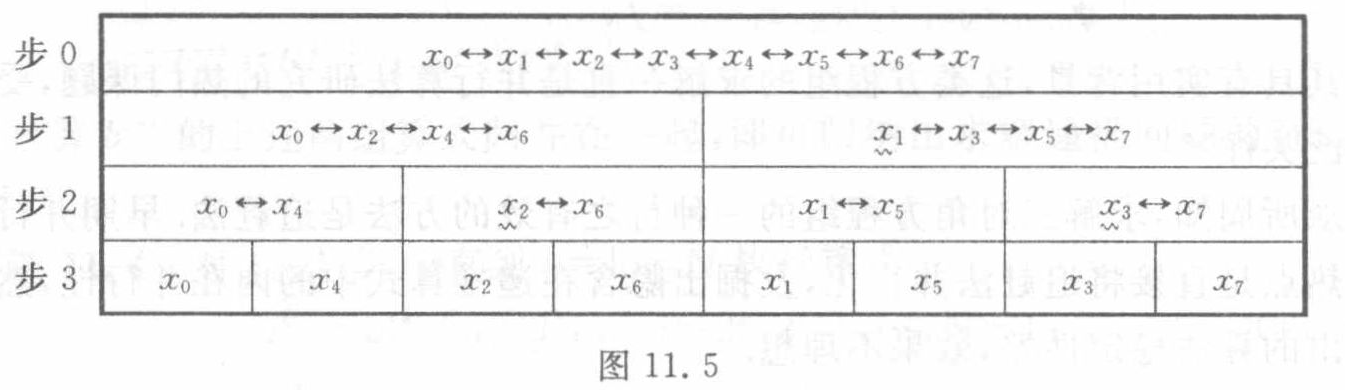
\includegraphics[width=0.85\linewidth,height=\textheight,keepaspectratio,alt={图 11.5（原图裁切）}]{../assets/ch11/figure-11-5.png}

图 11.5　原图逐层的步数标签、相关链与波纹线符号如下：

{\def\LTcaptype{none} % do not increment counter
\begin{longtable}[]{@{}
  >{\raggedright\arraybackslash}p{(\linewidth - 4\tabcolsep) * \real{0.3333}}
  >{\raggedright\arraybackslash}p{(\linewidth - 4\tabcolsep) * \real{0.3333}}
  >{\raggedright\arraybackslash}p{(\linewidth - 4\tabcolsep) * \real{0.3333}}@{}}
\toprule\noalign{}
\begin{minipage}[b]{\linewidth}\raggedright
原图步数标签
\end{minipage} & \begin{minipage}[b]{\linewidth}\raggedright
从左至右的相关链或单节
\end{minipage} & \begin{minipage}[b]{\linewidth}\raggedright
波纹线标记
\end{minipage} \\
\midrule\noalign{}
\endhead
\bottomrule\noalign{}
\endlastfoot
步 0 & \(x_0\leftrightarrow x_1\leftrightarrow x_2\leftrightarrow x_3\leftrightarrow x_4\leftrightarrow x_5\leftrightarrow x_6\leftrightarrow x_7\) & 无 \\
步 1 & \(x_0\leftrightarrow x_2\leftrightarrow x_4\leftrightarrow x_6\)；\(x_1\leftrightarrow x_3\leftrightarrow x_5\leftrightarrow x_7\) & \(x_1\) \\
步 2 & \(x_0\leftrightarrow x_4\)；\(x_2\leftrightarrow x_6\)；\(x_1\leftrightarrow x_5\)；\(x_3\leftrightarrow x_7\) & \(x_2,x_3\) \\
步 3 & \(x_0\)；\(x_4\)；\(x_2\)；\(x_6\)；\(x_1\)；\(x_5\)；\(x_3\)；\(x_7\) & 无 \\
\end{longtable}
}

（上表为原图标签与结构的文字转录。）

具体地说，其第 1 步将所给方程组（11.4.3）加工成两个子系统：

\begin{quote}
校注（agent 补充，CH11-E004）：式（11.4.2）第二行的首项在原图中印为 \(x_0\)，已照录。按照前文奇偶拆分、该行后续下标以及式（11.3.3）的相同链结构，此首项疑应为 \(x_1\)；属于原书排印疑误。
\end{quote}

\href{../../source-images/pdf-290.jpeg}{原页图像}

\[
\begin{cases}
b_0^{(1)}x_0+c_0^{(1)}x_2=f_0^{(1)},\\
a_2^{(1)}x_0+b_2^{(1)}x_2+c_2^{(1)}x_4=f_2^{(1)},\\
a_4^{(1)}x_2+b_4^{(1)}x_4+c_4^{(1)}x_6=f_4^{(1)},\\
a_6^{(1)}x_4+b_6^{(1)}x_6=f_6^{(1)};
\end{cases}
\]

\[
\begin{cases}
b_1^{(1)}x_1+c_1^{(1)}x_3=f_1^{(1)},\\
a_3^{(1)}x_0+b_3^{(1)}x_3+c_3^{(1)}x_4=f_3^{(1)},\\
a_5^{(1)}x_2+b_5^{(1)}x_5+c_5^{(1)}x_6=f_5^{(1)},\\
a_7^{(1)}x_4+b_7^{(1)}x_7=f_7^{(1)}.
\end{cases}
\]

它们分别对应于相关链 \(x_0\leftrightarrow x_2\leftrightarrow x_4\leftrightarrow x_6\) 与 \(x_1\leftrightarrow x_3\leftrightarrow x_5\leftrightarrow x_7\)（见图 11.5）。重复这种二分手续，第 2 步进一步加工出 4 个子系统：

\[
\begin{cases}
b_0^{(2)}x_0+c_0^{(2)}x_4=f_0^{(2)},\\
a_4^{(2)}x_0+b_4^{(2)}x_4=f_4^{(2)};
\end{cases}
\qquad
\begin{cases}
b_2^{(2)}x_2+c_2^{(2)}x_6=f_2^{(2)},\\
a_6^{(2)}x_2+b_6^{(2)}x_6=f_6^{(2)};
\end{cases}
\]

\[
\begin{cases}
b_1^{(2)}x_1+c_1^{(2)}x_5=f_1^{(2)},\\
a_5^{(2)}x_1+b_5^{(2)}x_5=f_5^{(2)};
\end{cases}
\qquad
\begin{cases}
b_3^{(2)}x_3+c_3^{(2)}x_7=f_3^{(2)},\\
a_7^{(2)}x_3+b_7^{(2)}x_7=f_7^{(2)}.
\end{cases}
\]

它们分别对应于相关链 \(x_0\leftrightarrow x_4\)，\(x_2\leftrightarrow x_6\)，\(x_1\leftrightarrow x_5\)，\(x_3\leftrightarrow x_7\)。最后，第 3 步将所给方程组（11.4.3）加工成如下形式：

\[
b_i^{(3)}x_i=f_i^{(3)},\quad i=0,1,\cdots,7.
\]

它对应于 8 条仅含一节的子链

\[
x_0,x_1,\cdots,x_7,
\]

从而立即得出所求的解

\[
x_i=f_i^{(3)}/b_i^{(3)},\quad i=0,1,\cdots,7.
\]

\begin{center}\rule{0.5\linewidth}{0.5pt}\end{center}

\subsection{相关原页校注（agent 补充）}\label{ux76f8ux5173ux539fux9875ux6821ux6ce8agent-ux8865ux5145}

以下校注来自本节覆盖的原页，可能也涉及同页相邻小节；原文照录与校正说明分开保留。

\subsubsection{原书 PDF 页 290 的校注}\label{ux539fux4e66-pdf-ux9875-290-ux7684ux6821ux6ce8}

\href{../pages/pdf-290.md}{完整原页转录} · \href{../../source-images/pdf-290.jpeg}{原页图像}

校注记录：CH11-E005, CH11-E006。

\begin{quote}
校注（agent 补充，CH11-E005）：本页第 1 步的第二个（奇数下标）子系统中，原书依次印有 \(a_3^{(1)}x_0\)、\(c_3^{(1)}x_4\)、\(a_5^{(1)}x_2\)、\(c_5^{(1)}x_6\)、\(a_7^{(1)}x_4\)，已据放大原图照录。按该页明确给出的奇数相关链，其变元依次应为 \(x_1,x_5,x_3,x_7,x_5\)；这里五个偶数下标与奇数子系统不相容，属原书下标疑误。
\end{quote}

\begin{quote}
校注（agent 补充，CH11-E006）：11.4.2 开头将``一般形式的三对角方程组''回引为（11.4.3），已照录。式（11.4.3）是 \(N=8\) 的示例，一般形式在式（11.4.1）；此处疑为原书交叉引用错误。
\end{quote}

\subsection{本节覆盖原页的校注记录}\label{ux672cux8282ux8986ux76d6ux539fux9875ux7684ux6821ux6ce8ux8bb0ux5f55}

下列记录按原页关联，含同页相邻小节的校注；计算时同时读取上文校注和完整原页。

\begin{itemize}
\tightlist
\item
  \texttt{CH11-E004}：原书 PDF 页 289
\item
  \texttt{CH11-E005}：原书 PDF 页 290
\item
  \texttt{CH11-E006}：原书 PDF 页 290, 291, 292
\end{itemize}

\end{document}
